\section{Database System}

The database system serves as the foundational framework for managing data storage, processing requests, delivering instructions in response to QR code scans, and it provides GUI tools for managing the database. It is essential for the functionality of various components, ensuring accurate and timely responses to user interactions. For instance, the localization system relies on the database to retrieve from it a QR code's global positions, while the customizable guidance system utilizes it to retrieve the latest instructions tailored for users. Several parts of the project depends on the database to keep data accurate and up-to-date. The database system is composed of the following components:
\subsection{Database}

The database serves as the backbone of the system, storing all data related to QR codes, building layouts, and navigation instructions. It is designed to organize QR code data in a manner that ensures each QR code is uniquely identifiable, allowing the mobile application to efficiently retrieve the correct information upon each scan.

\begin{figure}[h]
	\centering
	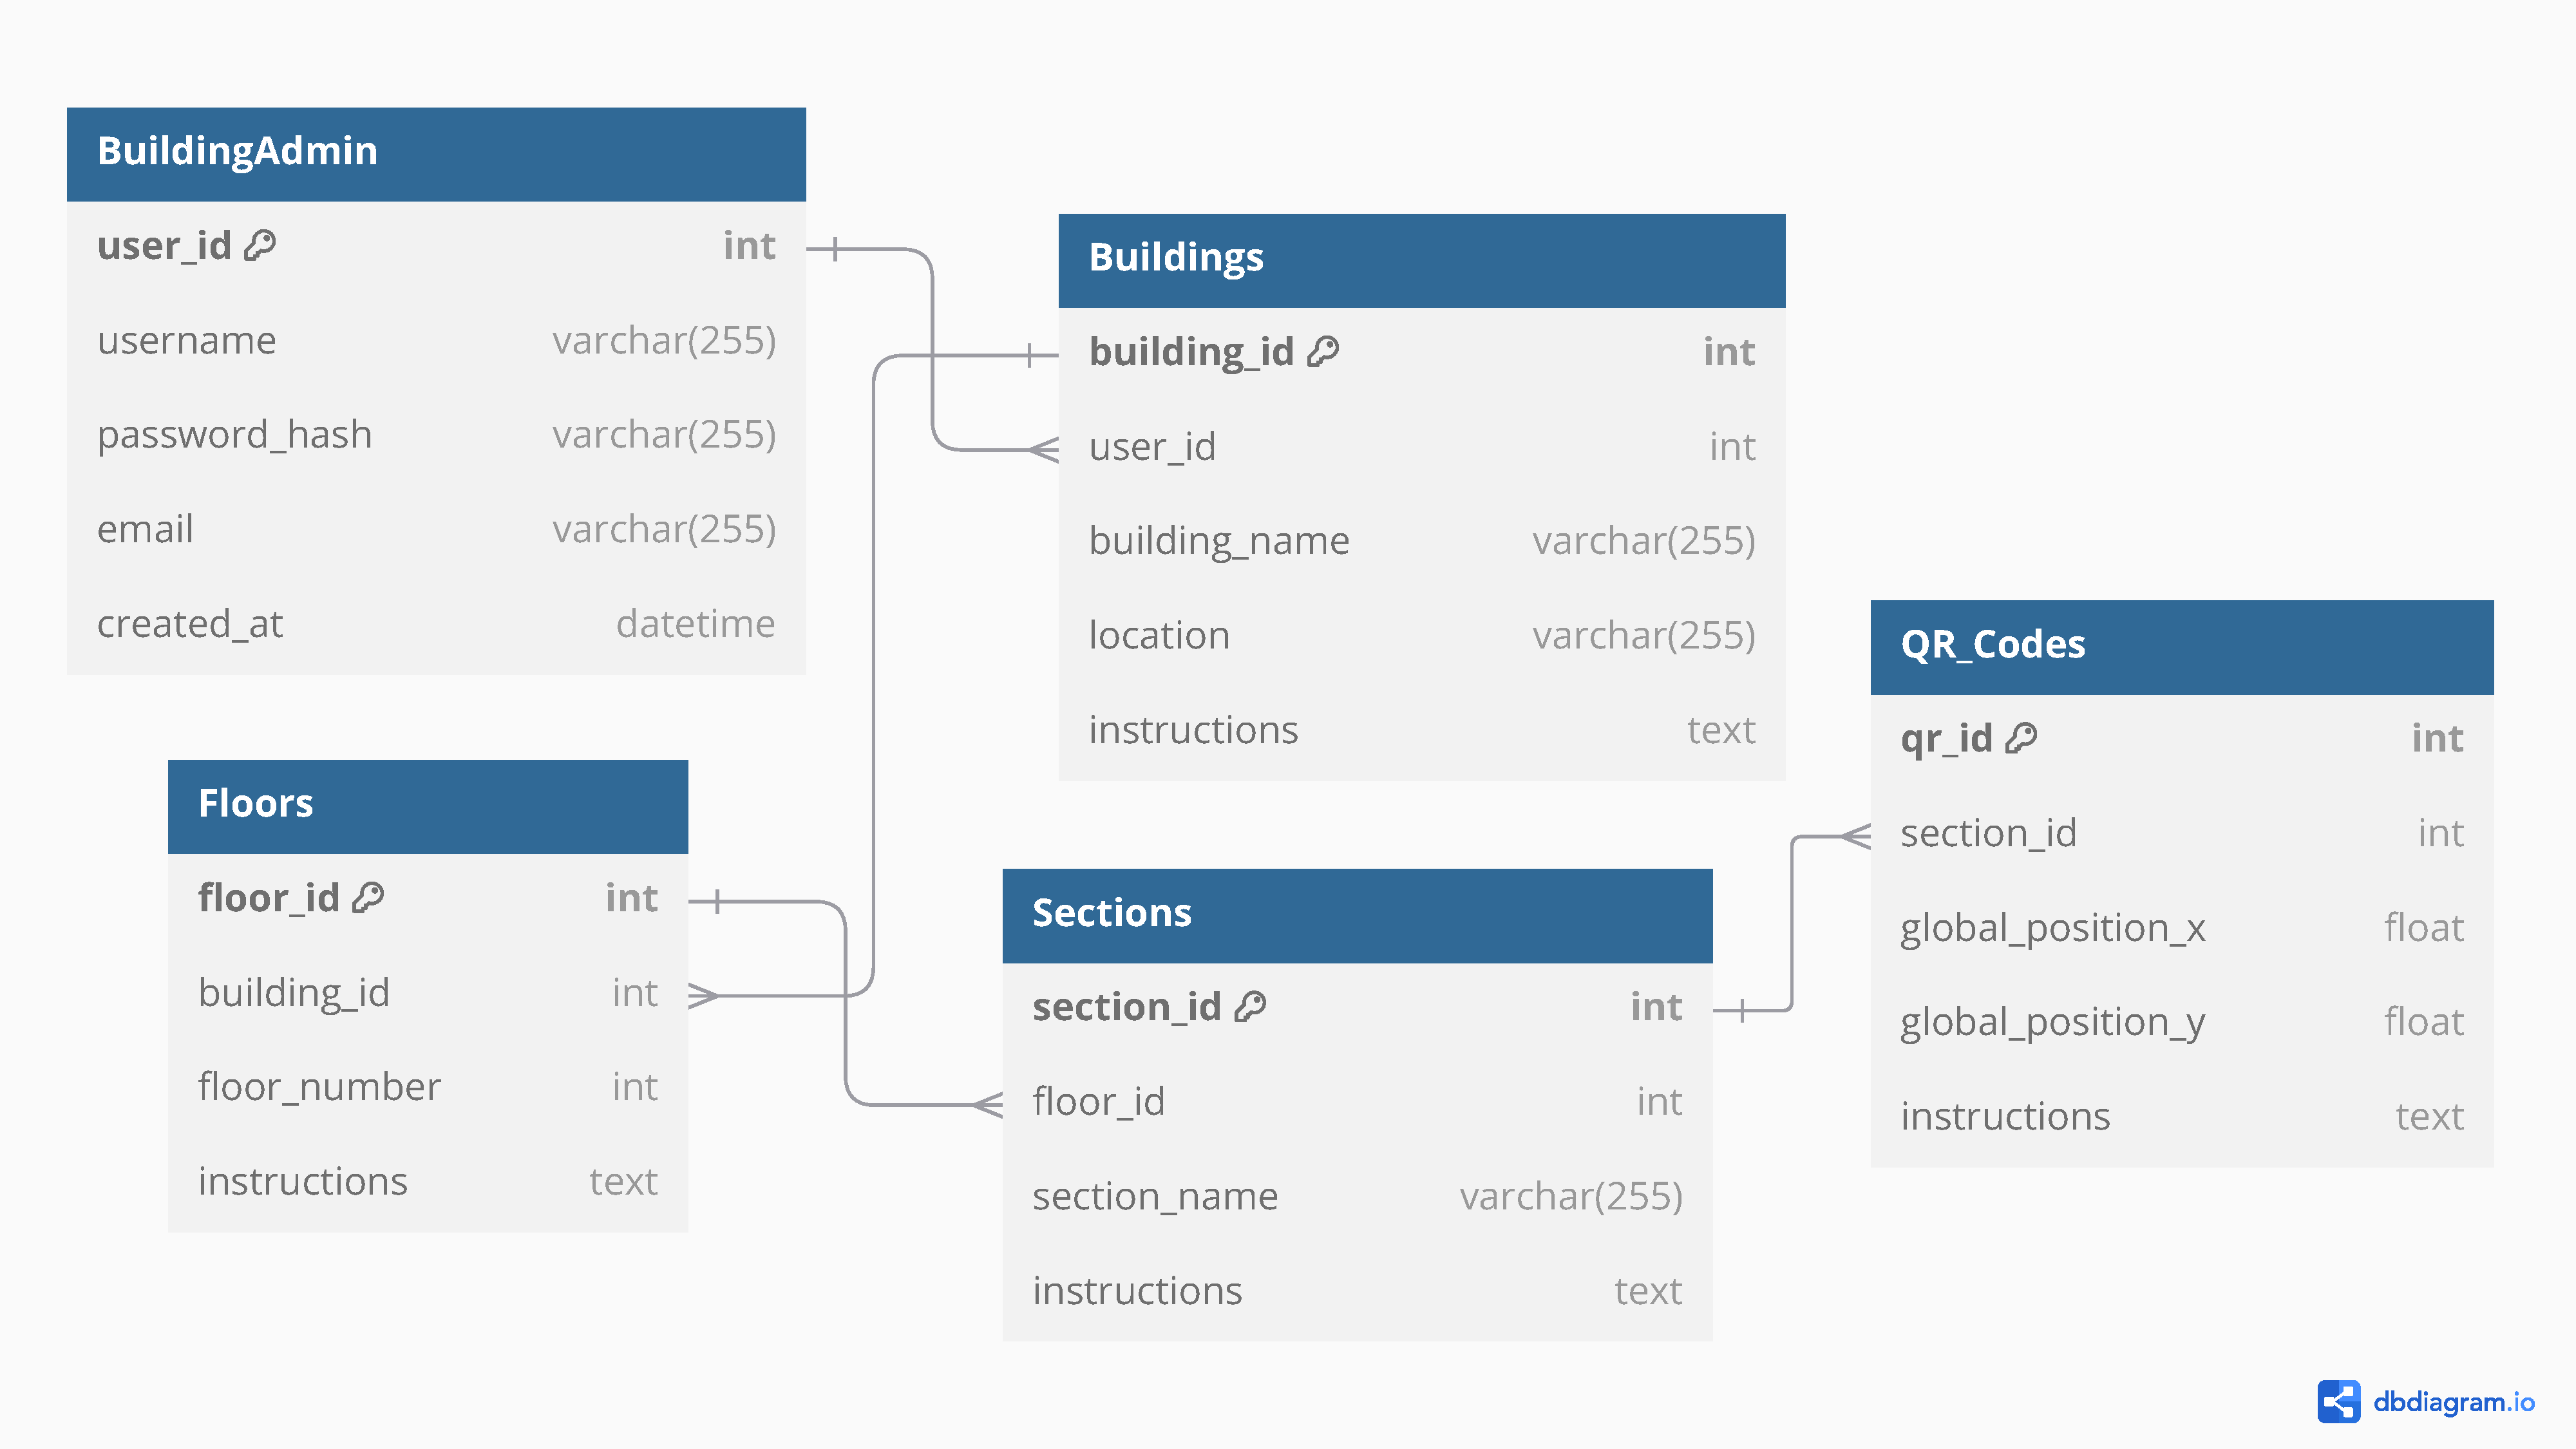
\includegraphics[width=1\linewidth]{assets/ch3/our_ERD}
	\caption{This Entity-Relationship Diagram (ERD) of Mosaned database}
	\label{fig:our_ERD}
\end{figure}

Figure \ref{fig:our_ERD} illustrates our database structure which is composed out of 5 main tables as follows:

\begin{itemize}
	\item \textbf{BuildingAdmin:}  
	\begin{itemize}
		\item \textbf{user\_id (Primary Key)}: A unique identifier for each user of the system, enabling individual management of buildings and associated data.
		\item \textbf{username}: The name chosen by the user for login purposes.
		\item \textbf{password\_hash}: A secure hash of the user's password used for authentication.
		\item \textbf{email}: The user's email address, utilized for notifications and account recovery.
		\item \textbf{created\_at}: A timestamp indicating when the user account was created.
	\end{itemize}
	
	\item \textbf{Buildings:}  
	\begin{itemize}
		\item \textbf{building\_id (Primary Key)}: A unique identifier for each building within the system.
		\item \textbf{user\_id (Foreign Key)}: Links the building to the associated user in the \texttt{BuildingAdmin} table, ensuring that each building is managed by the correct user.
		\item \textbf{building\_name}: The name of the building.
		\item \textbf{location}: The physical address or description of the building's location.
		\item \textbf{instructions}: General instructions related to the building, providing contextual information for navigation and management.
	\end{itemize}
	
	\item \textbf{Floors:}  
	\begin{itemize}
		\item \textbf{floor\_id (Primary Key)}: A unique identifier for each floor within a building.
		\item \textbf{building\_id (Foreign Key)}: Associates the floor with its corresponding building, establishing a clear hierarchical structure.
		\item \textbf{floor\_number}: Indicates the number of the floor (e.g., 1 for the first floor, 2 for the second, etc.).
		\item \textbf{instructions}: Specific instructions related to that floor, assisting users with effective navigation.
	\end{itemize}
	
	\item \textbf{Sections:}  
	\begin{itemize}
		\item \textbf{section\_id (Primary Key)}: A unique identifier for each section on a floor.
		\item \textbf{floor\_id (Foreign Key)}: Links the section to its respective floor, maintaining the organizational hierarchy.
		\item \textbf{section\_name}: The name or description of the section within the floor.
		\item \textbf{instructions}: Instructions specific to the section, enhancing the user’s ability to navigate the area.
	\end{itemize}
	
	\item \textbf{QR\_Codes:}  
	\begin{itemize}
		\item \textbf{qr\_id (Primary Key)}: A unique identifier for each QR code, ensuring no duplicates exist within the system.
		\item \textbf{section\_id (Foreign Key)}: Connects the QR code to its specific section.
		\item \textbf{global\_position\_x}: The X-coordinate representing the global position of the QR code.
		\item \textbf{global\_position\_y}: The Y-coordinate indicating the QR code's position, further aiding in navigation.
		\item \textbf{instructions}: Specific instructions directly linked to the QR code, providing targeted guidance for users when the QR code is scanned.
	\end{itemize}
\end{itemize}


\subsection{Building Management Dashboard}

The Building Management Dashboard is a web-based tool that allows building administrators to manage the indoor navigation system effectively. This dashboard provides an interface to control and update QR code instructions and manage QR codes within the building remotely.

Key features include:
\begin{itemize}
	\item \textbf{User Authentication:} Allows administrators to securely log in and access only their managed buildings.
	\item \textbf{Building and Floor Management:} Displays a list of buildings and their respective floors, allowing administrators to organize and view all QR codes assigned to each area.
	\item \textbf{QR Code Instruction Editing:} Administrators can add, update, or delete instructions for each QR code in the building, tailoring guidance to specific areas and ensuring data accuracy.
\end{itemize}

The dashboard enables efficient oversight and maintenance of QR code-based navigation, allowing real-time updates without modifying the physical QR codes.